\documentclass[11pt]{article}
\usepackage[T1]{fontenc}
\usepackage{listings}
\usepackage{float}

% Basic figure setup, for now with no caption control since it's done
% automatically by Pandoc (which extracts ![](path) syntax from Markdown).
\usepackage{graphicx}
\usepackage{caption}
\captionsetup[figure]{labelfont=bf}

\usepackage{xcolor} % Allow colors to be defined
\usepackage{geometry} % Used to adjust the document margins
\usepackage{amsmath} % Equations
\usepackage{amssymb} % Equations
\usepackage{textcomp} % defines textquotesingle
\usepackage{upquote} % Upright quotes for verbatim code
\usepackage{eurosym} % defines \euro
\usepackage[mathletters]{ucs} % Extended unicode (utf-8) support
\usepackage[utf8x]{inputenc} % Allow utf-8 characters in the tex document
\usepackage{fancyvrb} % verbatim replacement that allows latex
\usepackage{grffile} % extends the file name processing of package graphics 
% to support a larger range 
% The hyperref package gives us a pdf with properly built
% internal navigation ('pdf bookmarks' for the table of contents,
% internal cross-reference links, web links for URLs, etc.)
\usepackage{hyperref}
\usepackage{longtable} % longtable support required by pandoc >1.10
\usepackage{booktabs}  % table support for pandoc > 1.12.2
\usepackage[inline]{enumitem} % IRkernel/repr support (it uses the enumerate* environment)
\usepackage[normalem]{ulem} % ulem is needed to support strikethroughs (\sout)
% normalem makes italics be italics, not underlines
\usepackage{color}

\definecolor{codegreen}{rgb}{0,0.6,0}
\definecolor{codegray}{rgb}{0.5,0.5,0.5}
\definecolor{codepurple}{rgb}{0.58,0,0.82}
\definecolor{backcolour}{rgb}{0.95,0.95,0.92}

\lstdefinestyle{mystyle}{
	backgroundcolor=\color{backcolour},   
	commentstyle=\color{codegreen},
	keywordstyle=\color{magenta},
	numberstyle=\tiny\color{codegray},
	stringstyle=\color{codepurple},
	basicstyle=\footnotesize,
	breakatwhitespace=false,         
	breaklines=true,                 
	captionpos=b,                    
	keepspaces=true,                 
	numbers=left,                    
	numbersep=5pt,                  
	showspaces=false,                
	showstringspaces=false,
	showtabs=false,                  
	tabsize=2,
	linewidth=1.2\textwidth
}
\lstset{style=mystyle}


\title{%
	Dirichlet Process Mixture Models\\
	\large A tutorial and overview
}
\author{Guilherme Grijó Pires}
\date{}


% Setup hyperref package
\hypersetup{
	breaklinks=true,  % so long urls are correctly broken across lines
	colorlinks=true
}
% Slightly bigger margins than the latex defaults
\usepackage[parfill]{parskip}

\begin{document}


\maketitle

\section{Introduction}\label{introduction}

In this work I'll try to present the concept of Dirichlet Process and to
show how they can be used to implement Infinite Mixture Models. I'll
start by introducing the Dirichlet Distribution, the Dirichlet Process,
and the application of the Dirichlet Process to Infinite Mixture Models.
I'll then apply an implementation of this model to the clustering of
data, with an unknown number of clusters.
	
\section{Dirichlet Distribution}\label{dirichlet-distribution}
	
\subsection{An introduction}\label{an-introduction}

The Dirichlet Distribution is commonly used as the conjugate prior for
the Multinomial distribution. This means that for a Multinomial
likelihood model, the most natural/simple way to encode our prior
beliefs about the nature of the observations is by using a Dirichlet
distribution. Not only that, if we use a Dirichlet prior with a
Multinomial likelihood, the posterior will turn out to be a Dirichlet
distribution as well (obtained by updating the \(\boldsymbol\alpha\)
parameter's entries with the corresponding counts given by the
Multinomial observations).
	
Let \begin{eqnarray}
\boldsymbol\theta &=& (\theta_1 , \theta_2, ..., \theta_m) \nonumber \\
\boldsymbol\alpha &=& (\alpha_1 , \alpha_2, ..., \alpha_m) \nonumber
\end{eqnarray} Then \[\boldsymbol\theta \sim Dir(\boldsymbol\alpha) : 
P(\boldsymbol\theta)=\frac{\Gamma(\sum_{k}^{m} \alpha_k)}{\prod_{k}^{m}\Gamma(\alpha_k)}\prod_{k}^{m}\theta_{k}^{a_k -1}\]
	
Note that samples \(\boldsymbol\theta\) from the Dirichlet Distribution
belong to the probability simplex, which means
\(\sum_{k}^{m}\theta_k = 1, \theta_k \geq 0\)

The Dirichlet Distribution can be regarded as a distribution over
possible parameters for a Multinomial Distribution - which is the
intuitive reason to use the former as the latter's prior. Extending this
notion a bit further, we can regard the Dirichlet Distribution as a
distribution over (Multinomial) distributions.
	
\subsection{The $\boldsymbol{\alpha}$-effect}\label{the-boldsymbolalpha-effect}
	
Let's look at the effect of the \(\boldsymbol\alpha\) parameter on the
shape of the distribution. For simplicity, lets take \(m=3\). The
simplex of the corresponding space is a triangle and so it can be
projected to 2D and be easily plotted. See Figure 1 for plots of different
parameters and number of samples.
		
\begin{figure}
	\caption{The effect of the $\boldsymbol\alpha$ parameter on the Dirichlet Distribution}
	\makebox[\textwidth][c]{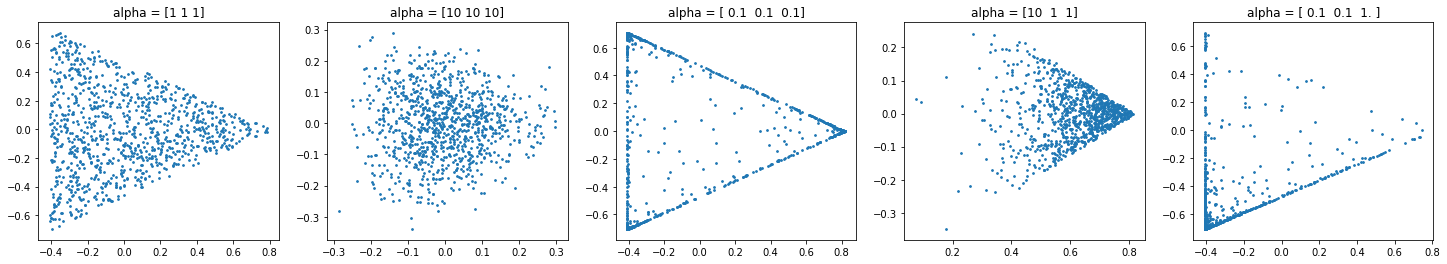
\includegraphics[width=1.2\textwidth]{output_8_0.png}}
\end{figure}
	
We see that \(\boldsymbol\alpha\) controls the nature of the probability
vectors sampled from the Dirichlet Distribution: 

\begin{itemize} 
	\item If the \(\alpha_i\) are all equal to \(\alpha\), the resulting samples 
	have a symmetric spread on the space. Particularly:
	\begin{itemize}
		\item If \(\alpha = 1\), the samples spread uniformely on the space
		\item If \(\alpha > 1\), dense (as in opposed to \emph{sparse}) samples are more frequent 
		\item If \(\alpha < 1\), sparse samples are more frequent
	\end{itemize}	
	\item If the \(\alpha_i\) are not equal, there will be a concentration of samples on either one 
	of the vertices or one of the edges of the space
\end{itemize}	
	
\section{Dirichlet Process}\label{dirichlet-process}
	
\subsection{Introduction to the concept}\label{introduction-to-the-concept}
	
The Dirichlet Process can be regarded as a generalization of the the
Dirichlet Distribution to infinite dimensions. It too defines a
distribution over distributions. However, while the Dirichlet
Distribution defines a distribution over random probability measures of
defined dimension, the Dirichlet Process defines a distribution over
random probability measures, of random dimension.
	
Formally:
	
\begin{itemize}
	\item Consider the measure space defined by \((\Theta, \Sigma)\), where
	\(\Theta\) is some set and \(\Sigma\) is a \(\sigma\)-algebra on
	\(\Theta\)
	\item Take a \emph{measurable finite partition} of \(\Theta\) :
	\(A_1, A_2, ..., A_k\)
	\item A Dirichlet Process is a random probability measure \(G\) over a
	measure space \((\Theta, \Sigma)\), that respects a special property:
		
	\begin{itemize}
		\item \([G(A_1), G(A_2), ..., G(A_3)] \sim Dir(\alpha H(A_1), \alpha H(A_2), ..., \alpha H(A_k))\)
	\end{itemize}
	\item The Dirichlet Process is parametrized by:
		
		\begin{itemize}
			\item \(\alpha \in \mathbb{R}\) : The concentration parameter
			\item \(H\) (a probability distribution): The base distribution
		\end{itemize}
		\item
		Most common notation: \(G \sim DP(\alpha, H)\)
\end{itemize}
	
Intuitively, \(H\) is the "mean distribution" and \(\alpha\) can be
regarded as an "inverse variance". A sample from a Dirichlet Process
will be an infinite sum of Dirac deltas, with different heights, and
with locations sampled from \(H\).
	
A somewhat counter-intuitive fact is that a sample \(G\) from a
Dirichlet Process will be discrete with probability 1, even if the base
distribution is smooth. Even so, the base distribution will be the mean
distribution!
	
\subsection{Posterior Inference}\label{posterior-inference}
	
Now suppose we use a (random) sample \(G\) from a \(DP\) as a likelihood
model for some i.i.d data \(\theta_1, \theta_2, ..., \theta_N\) :
\(\theta_n | G \sim G\).
	
Convenientely, the conjugacy of the Dirichlet Distribution to the
Multinomial Distribution still applies to the Dirichlet Process, which
means the posterior on \(G\) is also a Dirichlet Process and is given
(after some rather cumbersome algebraic manipulation) by:
\[ G | \theta_1, \theta_2, ..., \theta_N \sim DP(\alpha+N , \frac{\alpha H + \sum_{n=1}^{N}\delta_{\theta_n}}{\alpha+N}) \]
	
Where \(\delta_{\theta_n}\) is the Dirac delta function. (Note that some
of the \(\theta_n\) will fall on the same value, which means we'll have
summed \(\delta\)'s. A reasonable and intuitive way of thinking about
these, is as the counts of sampled \(\theta\) that fell on each value
(which hints at the empirical distribution).
	
The posterior predictive distribution of a DP is given by its base
distribution. Taking that fact, we see that the posterior predictive
distribution for \(\theta_{N+1}\) is:
\[\theta_{N+1} | \theta_1, ..., \theta_N \sim \frac{\alpha H + \sum_{n=1}^{N}\delta_{\theta_n}}{\alpha+N}\]
	
If you look carefully at that distribution, you'll see it has a smooth
part and a discrete part. Figure 2 presents a possible configuration for such a distribution.
	
\begin{figure}
	\centering
	\caption{Example of a DP posterior predictive function}
	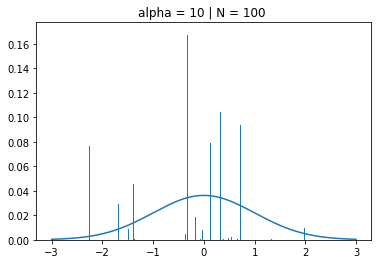
\includegraphics[width=0.5\textwidth]{output_19_0.png}
\end{figure}
	
That's rather unintuitive - how do you sample from such a distribution?
Hopefully the next section will make that clearer.
	
\subsubsection{Chinese Restaurant Process and Polya Urn Process}\label{chinese-restaurant-process-and-polya-urn-process}
	
Two very famous representations for the Dirichlet Process have been
devised, that evidence its clustering properties, in a \emph{rich get
richer} fashion. They are the Chinese Restaurant Process, and the Polya
Urn Process. Put simply, they provide a way to "implement" the posterior
predictive distribution I just presented, by either: - Assigning points
to an existing group, with some probability - Which corresponds to
assigning a person who just entered the restaurant to one of the
existing tables, in the Chinese Restaurant Process - And to add to the
urn a ball of the same color as some other ball sampled from the urn, in
the Polya Urn Process - Create a new group, based on the new point -
Which corresponds to assingning a person who just entered the restaurant
to an empty table, in the Chinese Restaurant Process - And to add a ball
of a new color to the urn, in the Polya Urn Model
	
This somewhat "dual" behaviour is evidenced by the posterior predictive
distribution, especially if we separate the expression in two terms:
\[\theta_{N+1} | \theta_1, ..., \theta_N \sim \frac{\alpha}{\alpha+N}H + 
\frac{N}{\alpha+N}(\frac{1}{N}\sum_{n=1}^{N}\delta_{\theta_n})\]
	
This way of writing the equation evidences the fact that the posterior
predictive distribution is a weighted sum of the base distribution and
the empirical distribution. How does one sample from such a
distribution? 
\begin{itemize}
	\item With probability \(\frac{\alpha}{N+\alpha}\) we sample
	the next \(\theta\) from the base distribution, \(H\)
	\item With probability
\(\frac{N}{N+\alpha}\) we sample the next \(\theta\) from the empirical
distribution
\end{itemize} 

As it is easy to see, as N increases (i.e. we see more data), the weight
of the base distribution becomes proportionally smaller - proper
Bayesian behaviour! - but the probability of a new (as in
\emph{previously unseen}) value for \(\theta\) is never \(0\). We can
also see that the concentration parameter will have control over the
final number of clusters: the bigger \(\alpha\) is, the likelier the
predictive distribution is to sample a new \(\theta\) value from the
base distribution. That can easily be observed by the plots portraied
on Figure 3.
	
	
\begin{figure}[H]
	\caption{Effect of the concentration parameter and the number of samples
		on the DP posterior predictive distribution}
	\makebox[\textwidth][c]{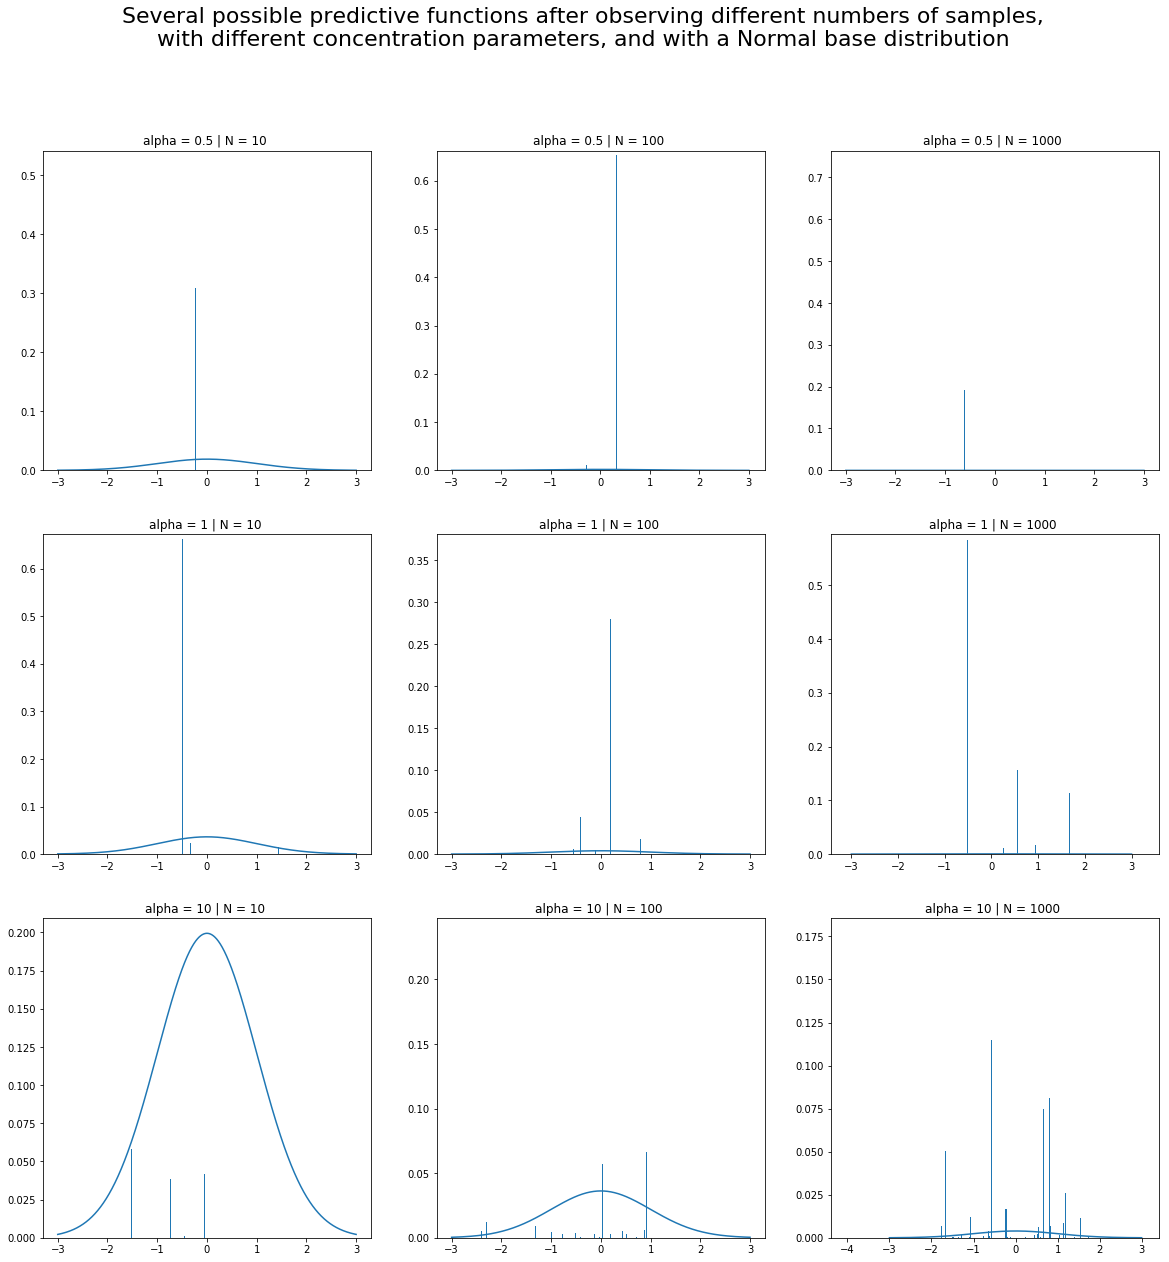
\includegraphics[width=0.9\textwidth]{output_23_0.png}}
\end{figure}
	
We can see these plots are coherent with the intuitive notion I hinted
at: for a fixed number of observed samples, a bigger \(\alpha\)
increases the weight of the base distribution; for a fixed \(\alpha\), a
bigger number of samples decreases the weight of the base distribution.
	
\subsubsection{Stick Breaking Representation}\label{stick-breaking-representation}
	
A third, more generative view of the DP, called the Stick Breaking
Representation allows us to obtains samples \(G\) from a Dirichlet
Process. It's important to keep in mind that samples \(G\) from a DP are
themselves probability distributions! The Stick Breaking Representation
obtains samples \(G \sim DP(\alpha, G)\) by the following process:
	
	\begin{itemize}
		\item
		Take a stick of length 1\\
		\item
		While remaining\_stick has length \textgreater{} 0:
		
		\begin{itemize}
			\item
			Sample a \(\pi_k\) from \(Beta(1,\alpha)\)
			
			\begin{itemize}
				\item
				Note that \(\pi_k \in [0,1]\)
			\end{itemize}
			\item
			Break the remaining stick at \(\pi_k\) of it's length\\
			\item
			current\_stick = first part, remaining\_stick = second part\\
			\item
			Sample a \(\theta_k\) from \(H\)
			\item
			Place a \(\delta_{\theta_k}\) with height = current\_stick on point
			\(\theta_k\)
		\end{itemize}
	\end{itemize}
	
We see that in the end of this process, G will be equal to \(\sum_{k=1}^\infty \delta_k \pi_k\) .
	
\subsection{An intuitive bridge to (Infinite) Mixture Models}\label{an-intuitive-bridge-to-infinite-mixture-models}
	
The usefulness of the DP in mixture models now starts to become
apparent. We can easily use the random variables \(\theta_k\) as the
latent "indexing" variables on a mixture model, taking advantage of the
natural clustering behaviour of the DP and also of the fact that, at any
point, it allows the possibility of seeing a new value for \(\theta_k\)
- hence the proneness to model a Mixture Model with an unknown number of
components: a new one can appear at any time, if the data so suggests.
	
Systematizing the Dirichlet Process Mixture Model: 
\begin{eqnarray}
	G|\alpha, H &\sim& DP(\alpha, H) \nonumber \\
	\theta_n|G &\sim& G \nonumber \\
	x_n|\theta_n &\sim& F(\theta_n) \nonumber
\end{eqnarray}
	
Where \(F(\theta_n)\) is a class conditional distribution, e.g., a
Gaussian in the case of a Gaussian Mixture Model.
	
One of the biggest motivations to use this kind of models lies in its
ability to directly attack the problem of model selection: there is no
initial assumption on the number of components, and the model itself
"searches" for the best possible.
	

\section{Inference in DPMM}\label{inference-in-dpmm}
	
Several ways of doing Inference on Dirichlet Process Mixture Models have
been proposed and shown. The most common ones involve Gibbs Sampling,
Collapsed Gibbs Sampling or other MCMC or simulation methods. More
recently some Variational methods have also been proposed. I will
present an overview of both approaches, also introducing the high-level
basics of Gibbs Sampling and Variational Inference.
	
Both of these approaches come from the need of computing complex (as in
\emph{complicated and hard}) integrals (usually on the denominators of
posterior distributions). Gibbs Sampling tackles this by sampling from
distributions that assymptotically approach the true ones, while
Variational methods work by converting the integral computation into an
optimization problem.
	
\subsection{Gibbs Sampling approach}\label{gibbs-sampling-approach}
\subsubsection{Gibbs Sampling}\label{gibbs-sampling}
	
As mentioned, Gibbs Sampling takes the approach of sampling from a
distribution that is assymptotically similar to the one of interest. It
is an instance of a broader class of sampling methods, called Markov
Chain Monte Carlo.
	
It's clear that if we had a black box from which we could take samples
of the distribution we care about, we could empirically estimate that
distribution. However, how can you build a black box for a distribution
you don't know yet?
	
First, there's the need to realize that what we actually want is to
compute something in the form of: \[E_{p(z)}[f(z)]=\int_{z}f(z)p(z)\]
Where \(p(z)\) governs the distribution of the values of \(z\), but the
integral we're actually interested is on the values of \(f(z)\).
Consider the previous expression in this form:
\[E_{p(z)}[f(z)]=\lim_{N \to \infty}\frac{1}{N}\sum_{N}f(z_{(i)})\]
	
Where \(z_{(i)}\) are observed values, taken from the \(p(z)\)
distribution. Here we're counting how many times \(f(z)\) landed on a
particular value and averaging it. So what we really want is to have a
way to "tell" how much time we spent on each "region" of the \(z\)-space
sow that we can accumulate \(f(z)\) values. A way to do so is to use a
Markov Chain that allows us to visit each \(z\)-value with a frequency
proportional to \(p(z)\) - hence the name Markov Chain Monte Carlo.
	
Gibbs Sampling is a way to implement such a Markov Chain. It's only
applicable when the \(z\)-space has at least 2 dimensions. It works by
getting each dimension of the next \(z\)-point individually, conditioned
on the remaining dimensions. For our models, these dimensions will be
parameters and variables.
	
Gibbs Samplers are derived on a per-model basis, because the way we
sample a new value for a dimension is determined by the way these
dimensions relate "interact" in the model.
	
\subsubsection{Collapsed Gibbs Sampling}\label{collapsed-gibbs-sampling}
	
Collapsed Gibbs Sampling takes the same principals from \emph{Vanilla}
Gibbs Sampling, but does the sampling of new dimension values with some
of the dimensions integrated out. This is made possible in some models
due to prior conjugacy and some algebraic tricks, and it makes the
sampler quicker because it reduces the number of variables per sampling
operation.
	
\subsubsection{Gibbs Sampling for DPMM}\label{gibbs-sampling-for-dpmm}
	
Several Gibbs Samplers have been devised for Dirichlet Process Mixture
Models. Although I'm not going to derive one here, I'll link some
references on that.
	
\subsection{Variational approach}\label{variational-approach}
	
\subsubsection{Variational Inference and Variational Bayes}\label{variational-inference-and-variational-bayes}
	
Variational Inference works by transforming the problem of integration
into one of optimization. It does so by fully replacing the distribution
we want to compute with an approximation which is chosen to live inside
of a distribution family. This family is commonly called a Variational
Family, and it doesn't necessarily include the real distribution
(actually, most likely it won't include the real distribution).
Variational Inference then proceeds by finding the parameters that
correspond to the optimal distribution in the Variational Family.
	
The question that should be ringing in your head now is: "Optimal
regarding what?". The answer is: We optimize the parameters so as to
minimize the Kullback-Leibler divergence between the true distribution
and the approximation. The KL divergence is a measure of how different
two distributions are. It's got its roots in Information Theory, and it
can be interpreted as the number of extra bits (if we work with base 2
logarithms) needed to encode an information source distributed according
to \(p\), if we use \(q\) to build our codebook.
	
A side note: the KL divergence is \textbf{not} symmetric, i.e.,
\(KL(p||q) \neq KL(q||p)\); in {[}{]} Murphy suggests that the reverse
version of the KL is statistically more sensible, but I won't go into
details on why that is. For the purpose of this overview, it suffices to
know that choosing to optimize for the forward KL divergence will yield
different results than choosing to optimize for the reverse KL
divergence.
	
Back on track. How does on go about computing the KL divergence between
two distributions without knowing one of them? The distribution we don't
know is precisely that which we want to estimate. It seems we got stuck
on an infinite loop. Alas! The whole trick of Variational Inference is
the way to break this loop. It turns out there's a way to leverage some
probability equalities and Jensen's inequality to come up with an
expression, called the Expectation Lower Bound, ELBO. Maximizing this
expression is equivalent to minimizing the KL divergence without needing
to know a closed form for \(p(x)\). Here's the derivation of that
result:
	
Consider Jensen's inequality (applied to Expectation):
\[f(E[X]) \geq E[f(X)]\]
	
Applying it to the log-probability of the observations:
\begin{eqnarray}
	log\ p(x) &=& log \int_z p(x,z) dz \nonumber \\
	&=& log \int_z p(x,z)\frac{q(z)}{q(z)} dz \nonumber \\
	&=& log E_q[\frac{p(x,Z)}{q(z)}] \nonumber \\
	&\geq& E_q[log\ p(x,Z)] - E_q[log\ q(Z)] \nonumber 
\end{eqnarray}
	
Our goal is now to find the parameters that yield the \(q(Z)\)
distribution that makes this bound as tight as possible. One of the
advantages of Variational methods as compared to sampling methods is the
fact that this optimization yields deterministic results, and
Variational methods are faster in general. However there's usually an
accuracy trade-off.
	
You might have noticed that the title for this section includes
"Variational Bayes". This refers to the application of Mean-Field
Variational Inference, where the Variational distribution is of the form
\(\prod_i q_i(x_i)\)
	
\subsubsection{Streaming Variational Bayes and DPMM}\label{streaming-variational-bayes-and-dpmm}
	
Streaming Variational Bayes is a framework by \emph{Broderick, et al.}
that proposes a way to leverage the conjugacy of some distributions to
allow the fitting of the approximation to be computed in a streaming
fashion - which aligns with the current tendencies of big-data and
scalability. This framework has been leveraged by \emph{Huynh et al.} to
apply Variational Inference to Dirichlet Process Mixture Models.
	
	
\section{Experiments}\label{experiments}

I used the BayesianGaussianMixture implementation from
\href{scikit-learn.org}{scikit-learn} to find clusters of countries with
similar living standards.
\href{http://www.sharecsv.com/s/4165c9b03d9fffdef43a3226613ff37c/Countries.csv}{Here}
is the dataset I used. The code used to generate this figure can be found on the Appendix section.


\begin{figure}[H]
	\centering
	\caption{Clustering data about countries' living standards}
		\makebox[\textwidth][c]{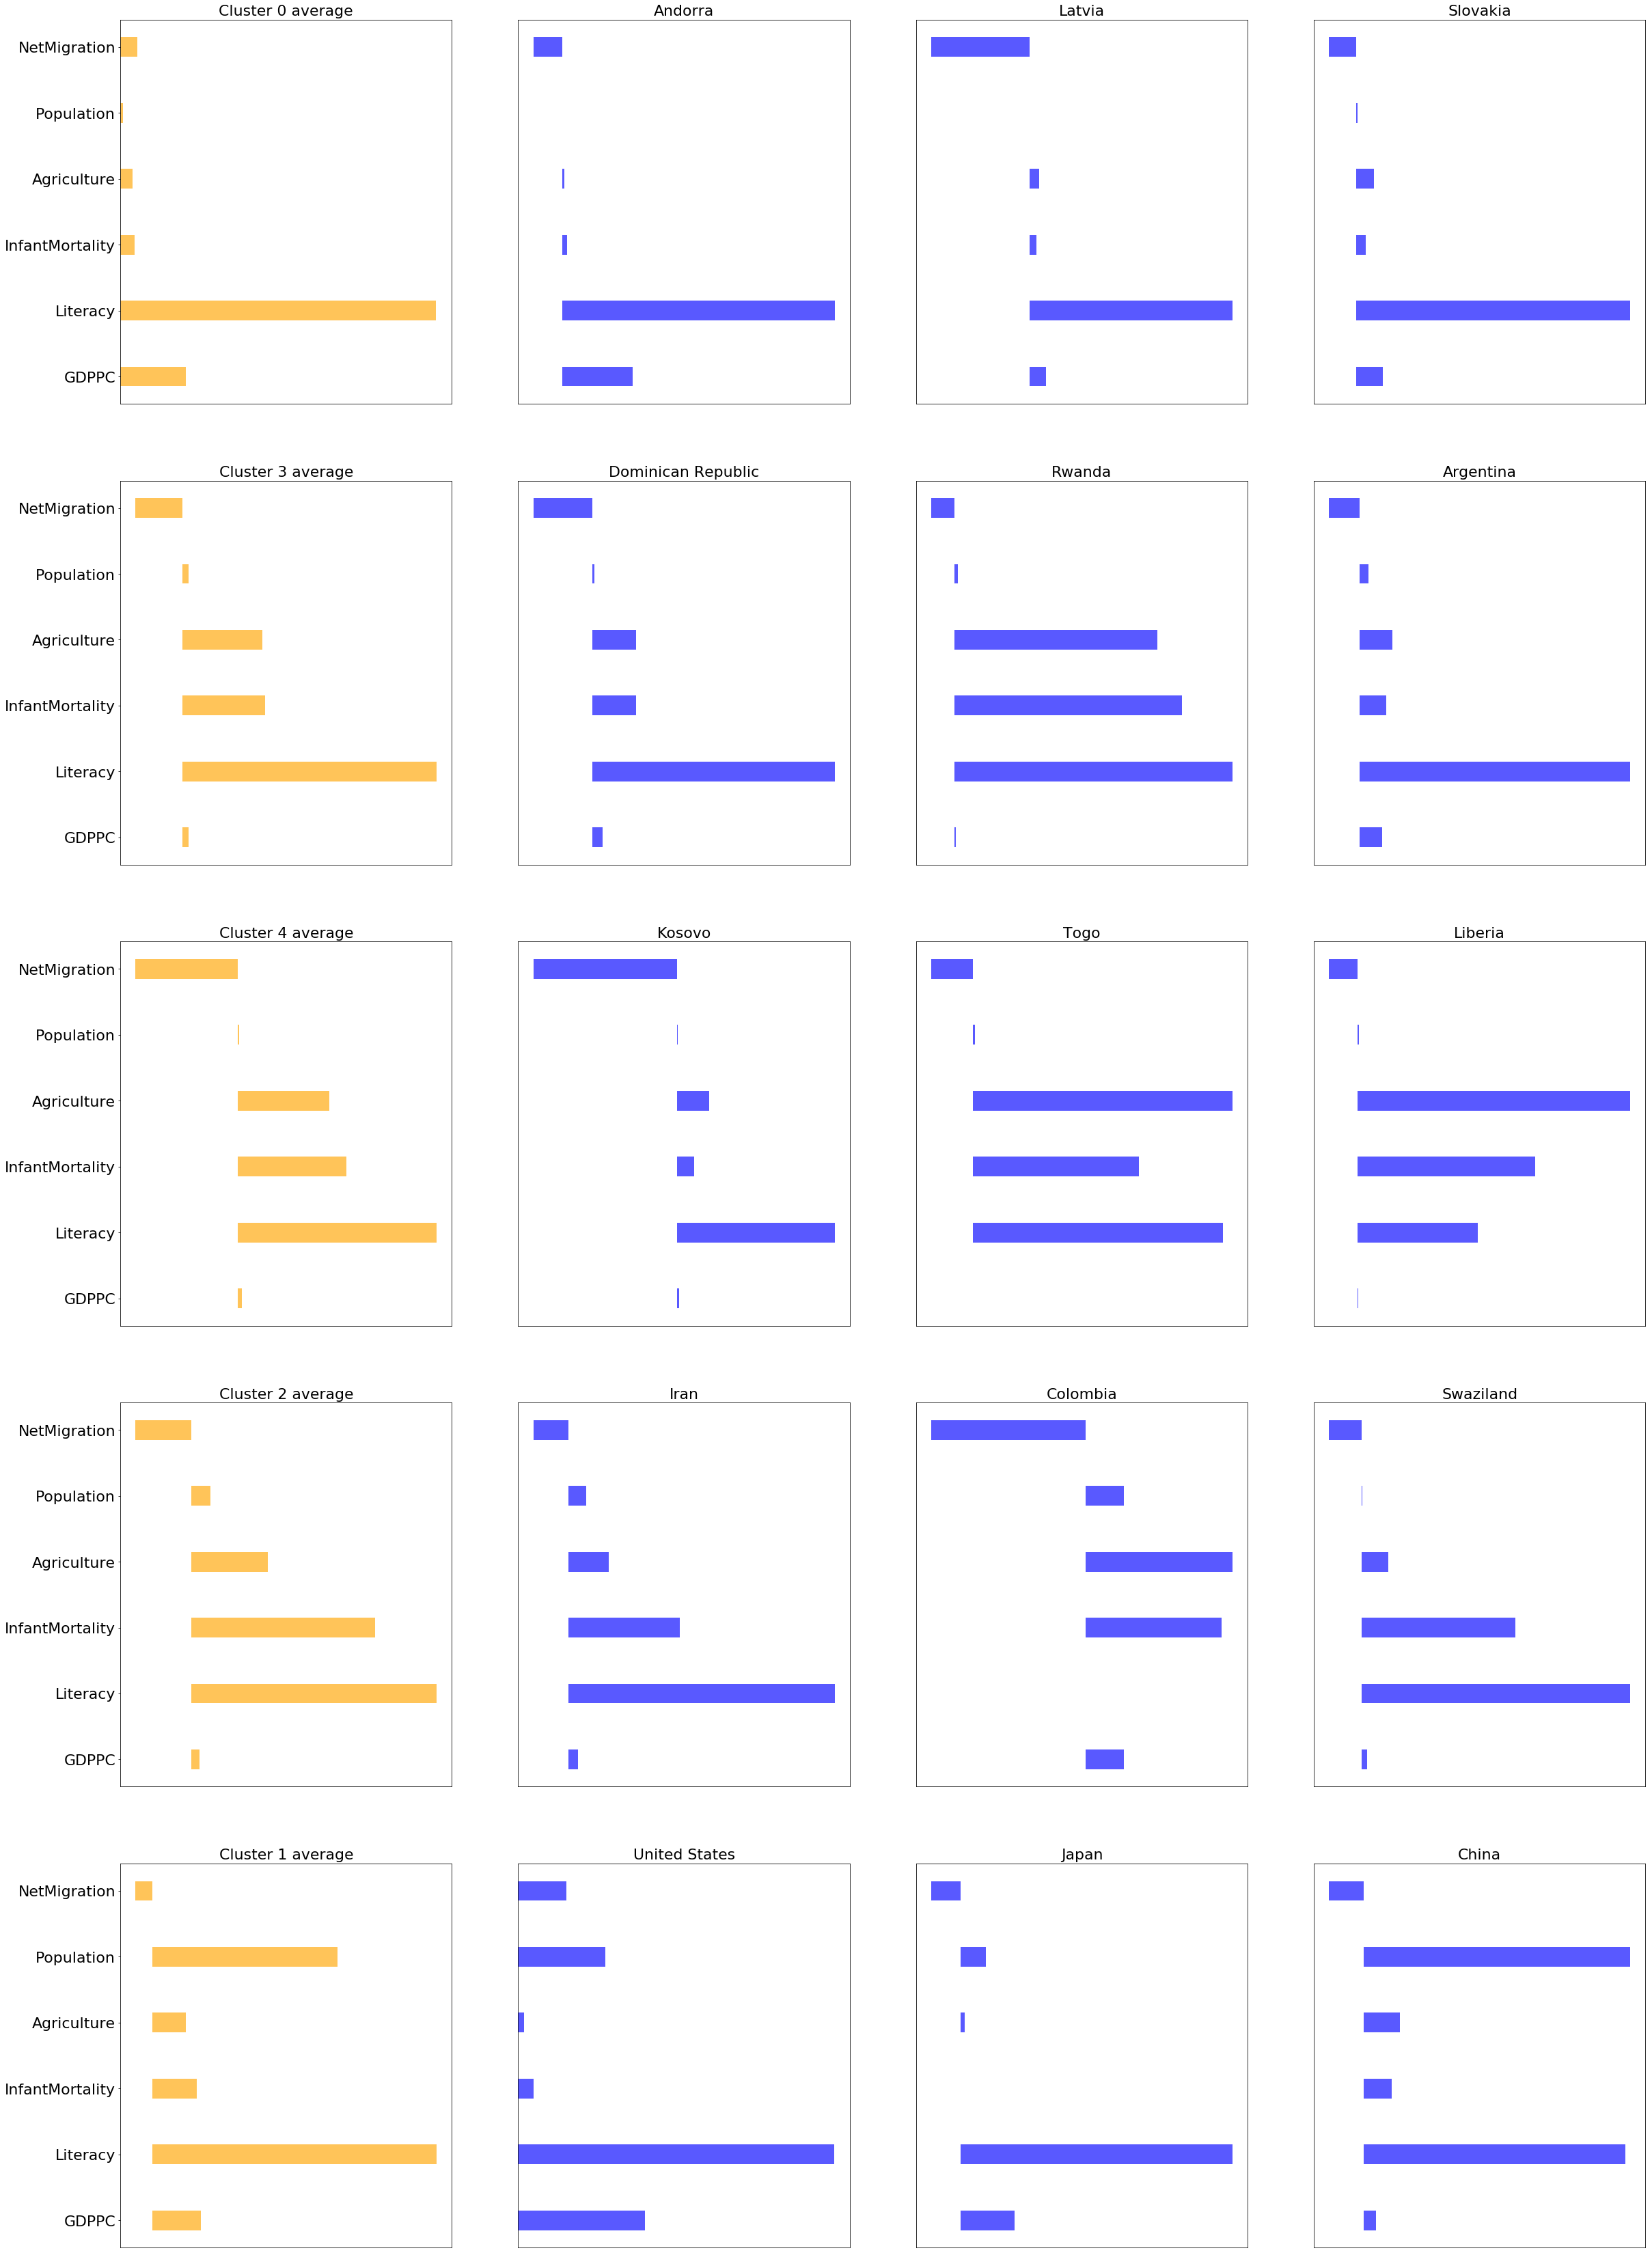
\includegraphics[width=1.1\textwidth]{output_60_0.png}}
\end{figure}
	
\section{Suggestions for future research}\label{proposals-for-future-research}
	
One direction of research I feel tempted to follow is the application of
Neural Variational Inference as an alternative to classic Variational
Inference and MCMC methods for fitting Dirichlet Process Mixture Models.
Neural Variational Inference has been applied with particular success to
language modelling and other text processing tasks - which are areas
where DPMM are traditionally applied (for instance in Latent Dirichlet
Allocation) - and it aligns with the current trend of leveraging Deep
Learning. Adversarial Networks have also been used with good results to
model complex probabilistic distribution, so perhaps applying them to
DPMMs can also be an interesting research premise.
	
	
\nocite{*}
\bibliographystyle{abbrv}
\bibliography{dpmm}
	
	
\section*{Appendix}
\subsection{Code to generate Figure 1}
\begin{lstlisting}[language=Python]
import numpy as np
import matplotlib.pyplot as plt

from scipy.stats import dirichlet as Dir

ortog = (1/np.sqrt(3)) * np.ones(3)
	
x = np.array([1,0,0])
x = x - np.dot(x, ortog) * ortog
x /= np.linalg.norm(x)
y = np.cross(ortog, x)
	
def project3dsample(sample):
	return np.array([np.dot(sample, x), np.dot(sample, y)])
	
fig, axs = plt.subplots(1,5, figsize=(25,4))
	
alphas = [
	np.array([1,1,1]),
	np.array([10,10,10]),
	np.array([0.1,0.1,0.1]),
	np.array([10,1,1]),
	np.array([0.1,0.1,1])
]
	
for alpha, ax in zip(alphas, axs):
	samples = np.array(
	[project3dsample(sample) for sample in Dir.rvs(alpha, size=1000)])
	ax.set_title("alpha = {}".format(alpha))
	ax.scatter(samples[:,0], samples[:,1], s=3);
	
plt.show()
\end{lstlisting}

\subsection{Code to generate Figure 2}
\begin{lstlisting}[language=Python]
from scipy.stats import beta
from scipy.stats import norm

def predictive_posterior_plot(N, alpha, ax):
	stick = 1
	pis = []
	for i in range(N):
		pi = stick * beta.rvs(1, alpha)
		pis.append(pi)
		stick -= pi

	pis = np.array(pis)*N/(alpha+N)
	thetas = norm.rvs(size=N)
	x = np.array(range(-3000,3000))*0.001
	y = norm.pdf(x)*alpha/(alpha+N)

	ax.set_title("alpha = {} | N = {} ".format(alpha, N))
	ax.plot(x,y)
	ax.set_ylim((0,max([max(pis),max(y)])+0.01))
	ax.bar(thetas,pis,0.01)

fig, ax = plt.subplots()
predictive_posterior_plot(100,10,ax)
plt.show()
\end{lstlisting}

\subsection{Code to generate Figure 3}
\begin{lstlisting}[language=Python]
import itertools

fig, axs = plt.subplots(3,3, figsize=(20,20))

alphas = [0.5, 1, 10]
Ns = [10, 100, 1000]
axs = axs.flatten()

for (ax, (alpha, N)) in zip(axs, itertools.product(alphas, Ns)):
	predictive_posterior_plot(N, alpha, ax)

plt.suptitle("Several possible predictive functions after observing different numbers of samples,\n"+
"with different concentration parameters, and with a Normal base distribution", fontsize=22)

plt.show()
\end{lstlisting}

\subsection{Code to generate Figure 4}
\begin{lstlisting}[language=Python]
import pandas as pd
df = pd.read_csv("./Countries.csv")

cols_of_interest = ["GDPPC", "Literacy", "InfantMortality", "Agriculture", "Population", "NetMigration"]
y = df[cols_of_interest].values

from sklearn.mixture import BayesianGaussianMixture

m = BayesianGaussianMixture(
	n_components=5, 
	weight_concentration_prior=1/5, #alpha
	weight_concentration_prior_type="dirichlet_process",
	max_iter=10000,
	init_params="random"
)

m.fit(y)
preds = m.predict(y)
print(np.bincount(preds))


grouped = dict(zip(range(0,100), [list() for _ in range(0,100)]))

for i in range(len(preds)):
	grouped[preds[i]].append(df.iloc[i]["Name"])

to_del = []
for key in grouped:
	if len(grouped[key]) == 0:
		to_del.append(key)

for key in to_del:
	del grouped[key]
	
from sklearn.preprocessing import MinMaxScaler

for col in cols_of_interest:
	if col != "NetMigration":
		df[col] = MinMaxScaler(feature_range=(0,1)).fit_transform(df[col].values.reshape(-1,1))
	else:
		df[col] = MinMaxScaler(feature_range=(-1,1)).fit_transform(df[col].values.reshape(-1,1))

def plot_country(ax, country, cluster_key=None):
	x = np.arange(len(cols_of_interest))

	if cluster_key != None:
		rows = df.loc[df["Name"].isin(grouped[cluster_key])][cols_of_interest].values
		y = np.mean(rows, axis=0)
		country = "Cluster {} average".format(cluster_key)
		ax.set_yticks(x)
		ax.set_yticklabels(cols_of_interest, fontsize=22)
		color="orange"
	else:
		y = df.loc[df["Name"] == country][cols_of_interest].values.flatten()
		ax.tick_params(axis="y", which="both", left="off", right="off", labelleft="off")
	color="blue"

	ax.tick_params(axis="x", which="both", bottom="off", top="off", labelbottom="off")
	ax.set_title(country, fontsize=22)
	ax.barh(x, y, height=0.3, alpha=0.65, color=color)


def plot_cluster(axs, key):
	countries = np.random.choice(grouped[key], size=3, replace=False)
	for ax, country in zip(axs[1:4], countries):
		plot_country(ax, country)
		
	plot_country(axs[0],"", key)
	
fig, axs_ = plt.subplots(5,4,figsize=(40,60))

top_5 = sorted(grouped.items(), key=lambda x: len(x[1]), reverse=True)[:5]

for (cluster,_), axs in zip(top_5, axs_):
	plot_cluster(axs, cluster)

plt.show() 
\end{lstlisting}

\end{document}